

\chapter{Double Scenario Classification of the first and last shared app, KFold Validation}

Starting with fitting randomly the classifiers, there are some statistics of the data used for the first test: \\
 {\def\arraystretch{1.3} 
 \begin{table}[H] 
\centering 
\begin{tabular}{|l|l|l|} 
\hline 
  &count train  &count test  \\ \hline
mess\_mess  &96  &254  \\ \hline
tele\_mess  &99  &251  \\ \hline
what\_mess  &107  &243  \\ \hline
mess\_tele  &98  &252  \\ \hline
tele\_tele  &111  &239  \\ \hline
what\_tele  &105  &245  \\ \hline
mess\_what  &116  &234  \\ \hline
tele\_what  &103  &247  \\ \hline
what\_what  &121  &229  \\ \hline
original  &94  &256  \\ \hline
\end{tabular} 
\end{table} }
\section{Logistic regression results:} 
Confusion matrix with number of sample and with normalization:
 {\def\arraystretch{1.3} 
 \begin{table}[H] 
\centering 
\begin{tabular}{|l|l|l|l|l|l|l|l|l|l|l|} 
\hline 
  &m\_m  &m\_t  &m\_w  &t\_m  &t\_t  &t\_w  &w\_m  &w\_t  &w\_w  &original  \\ \hline
mess\_mess  &248  &5  &1  &0  &0  &0  &0  &0  &0  &0  \\ \hline
tele\_mess  &2  &233  &14  &0  &0  &0  &2  &0  &0  &0  \\ \hline
what\_mess  &13  &26  &202  &0  &0  &2  &0  &0  &0  &0  \\ \hline
mess\_tele  &0  &0  &0  &65  &116  &3  &0  &68  &0  &0  \\ \hline
tele\_tele  &0  &0  &0  &66  &57  &2  &0  &114  &0  &0  \\ \hline
what\_tele  &0  &0  &0  &3  &4  &235  &1  &2  &0  &0  \\ \hline
mess\_what  &0  &0  &0  &1  &0  &1  &80  &0  &152  &0  \\ \hline
tele\_what  &0  &0  &0  &65  &129  &3  &0  &50  &0  &0  \\ \hline
what\_what  &0  &0  &0  &0  &0  &0  &104  &0  &123  &2  \\ \hline
original  &0  &0  &0  &0  &0  &0  &0  &0  &5  &251  \\ \hline
\end{tabular} 
\end{table} }

 \begin{figure}[H] 
\centering 
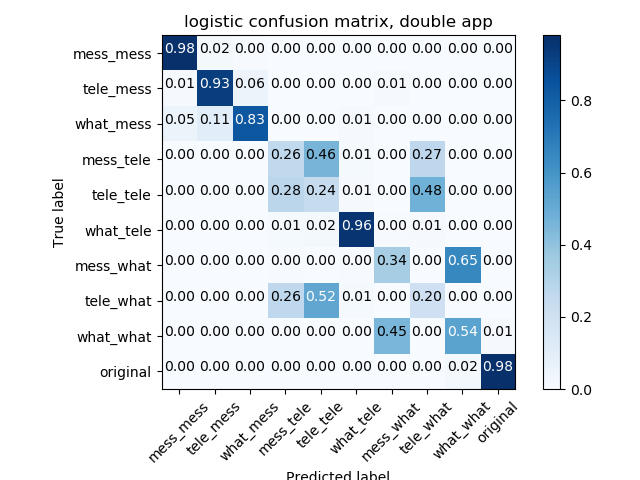
\includegraphics[scale=.6]{images/new_met_lr_initial_double_complete.png} 
\caption{logistic regression, last app classified} 
\end{figure} 


Result of the KFold validation with 10 bins:
 {\def\arraystretch{1.3} 
 \begin{table}[H] 
\centering 
\begin{tabular}{|l |l |l |l |l |l |l |l |l |l |}  
\hline 
0.6000&
0.5619&
0.6381&
0.6095&
0.6190&
0.6667&
0.6000&
0.5810&
0.5429&
0.6190\\ \hline  

\end{tabular} 
\end{table} }

The mean is : 0.603810\section{Linear Support Vector Machine results:} 
Confusion matrix with number of sample and with normalization:
 {\def\arraystretch{1.3} 
 \begin{table}[H] 
\centering 
\begin{tabular}{|l|l|l|l|l|l|l|l|l|l|l|} 
\hline 
  &m\_m  &m\_t  &m\_w  &t\_m  &t\_t  &t\_w  &w\_m  &w\_t  &w\_w  &original  \\ \hline
mess\_mess  &244  &5  &2  &0  &2  &0  &0  &0  &1  &0  \\ \hline
tele\_mess  &1  &217  &14  &3  &2  &0  &10  &1  &3  &0  \\ \hline
what\_mess  &14  &17  &192  &3  &0  &1  &9  &4  &3  &0  \\ \hline
mess\_tele  &0  &0  &0  &68  &106  &5  &1  &71  &1  &0  \\ \hline
tele\_tele  &0  &1  &0  &64  &49  &4  &0  &121  &0  &0  \\ \hline
what\_tele  &0  &0  &0  &4  &4  &234  &1  &2  &0  &0  \\ \hline
mess\_what  &0  &0  &0  &2  &1  &0  &83  &0  &148  &0  \\ \hline
tele\_what  &0  &1  &0  &61  &131  &5  &0  &49  &0  &0  \\ \hline
what\_what  &0  &0  &0  &1  &1  &0  &101  &1  &125  &0  \\ \hline
original  &0  &0  &0  &2  &1  &0  &0  &0  &5  &248  \\ \hline
\end{tabular} 
\end{table} }

 \begin{figure}[H] 
\centering 
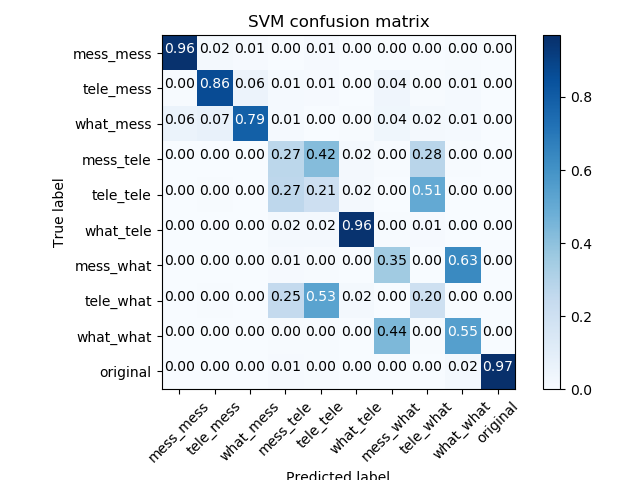
\includegraphics[scale=.6]{images/new_met_lsvm_initial_double_complete.png} 
\caption{linear SVM, last app classified} 
\end{figure} 


Result of the KFold validation with 10 bins:
 {\def\arraystretch{1.3} 
 \begin{table}[H] 
\centering 
\begin{tabular}{|l |l |l |l |l |l |l |l |l |l |}  
\hline 
0.6000&
0.5429&
0.6095&
0.5810&
0.6000&
0.7048&
0.6381&
0.6000&
0.5810&
0.6190\\ \hline  

\end{tabular} 
\end{table} }

The mean is : 0.607619\section{Random forest results:} 
Confusion matrix with number of sample and with normalization:
 {\def\arraystretch{1.3} 
 \begin{table}[H] 
\centering 
\begin{tabular}{|l|l|l|l|l|l|l|l|l|l|l|} 
\hline 
  &m\_m  &m\_t  &m\_w  &t\_m  &t\_t  &t\_w  &w\_m  &w\_t  &w\_w  &original  \\ \hline
mess\_mess  &236  &7  &9  &0  &0  &0  &0  &0  &1  &1  \\ \hline
tele\_mess  &13  &214  &24  &0  &0  &0  &0  &0  &0  &0  \\ \hline
what\_mess  &24  &21  &188  &0  &0  &0  &2  &0  &5  &3  \\ \hline
mess\_tele  &0  &0  &0  &32  &116  &3  &0  &101  &0  &0  \\ \hline
tele\_tele  &0  &0  &0  &72  &46  &4  &0  &117  &0  &0  \\ \hline
what\_tele  &0  &0  &0  &1  &2  &239  &0  &3  &0  &0  \\ \hline
mess\_what  &1  &0  &0  &0  &0  &0  &70  &0  &163  &0  \\ \hline
tele\_what  &0  &0  &0  &71  &128  &5  &0  &43  &0  &0  \\ \hline
what\_what  &0  &0  &0  &0  &0  &0  &127  &0  &98  &4  \\ \hline
original  &0  &0  &0  &0  &0  &1  &0  &0  &1  &254  \\ \hline
\end{tabular} 
\end{table} }

 \begin{figure}[H] 
\centering 
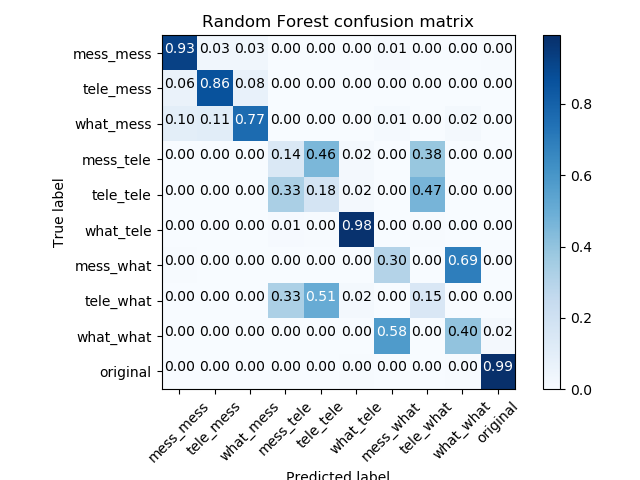
\includegraphics[scale=.6]{images/new_met_rf_initial_double_complete.png} 
\caption{random forest, last app classified} 
\end{figure} 


Result of the KFold validation with 10 bins:
 {\def\arraystretch{1.3} 
 \begin{table}[H] 
\centering 
\begin{tabular}{|l |l |l |l |l |l |l |l |l |l |}  
\hline 
0.5333&
0.5048&
0.6095&
0.5238&
0.5810&
0.5905&
0.5714&
0.6286&
0.5524&
0.5619\\ \hline  

\end{tabular} 
\end{table} }

The mean is : 0.565714